\chapter{Attacchi alle reti e fondamenti di crittografia}

% ══════════════════════════════════════════════════════════════
\section{Perché la sicurezza di rete}
% ══════════════════════════════════════════════════════════════

La pila è completa, dall'applicazione al filo, e finora ogni protocollo che abbiamo visto si è fidato di chi stava dall'altra parte.
Buona parte di essa fu progettata per qualche migliaio di utenti che si conoscevano; oggi porta le nostre credenziali, il nostro
denaro e i nostri dati sanitari. Nella tabella dei protocolli applicativi, accanto a HTTP, SMTP, Telnet e FTP c'era un gemello
\emph{sicuro} (HTTPS, SMTPS, SSH, FTPS): in questo capitolo vediamo che cosa voglia dire ``sicuro''. Prima gli \textbf{attacchi}, cioè
che cosa può fare davvero un avversario sulla rete; poi le \textbf{proprietà} che una comunicazione sicura deve avere, una per
attacco; infine la \textbf{crittografia} che le fornisce, dai cifrari di duemila anni fa a quelli del browser.

\dfn{Sicurezza di rete}{
    La \textbf{sicurezza di rete} è il campo che studia i possibili \textbf{attacchi} alle reti e i modi per \textbf{prevenirli}.
}

\begin{itemize}
    \item Le reti fanno parte della nostra vita (la connessione a Internet è considerata quasi come l'acqua o la corrente), e una grande
          quantità dei nostri dati sensibili viaggia in rete.
    \item Esistono molti tipi di attacchi, con scopi e meccanismi diversi.
    \item Gli attacchi evolvono insieme alla tecnologia e al pubblico delle reti.
    \item La maggior parte combina quattro mosse: \textbf{esplorare} (le scansioni di porte che abbiamo visto), \textbf{ascoltare},
          \textbf{impersonare}, \textbf{interrompere}.
\end{itemize}

% ══════════════════════════════════════════════════════════════
\section{I malware}
% ══════════════════════════════════════════════════════════════

\dfn{Malware}{
    Un \textbf{malware} è un software malevolo che può arrivare su un computer attraverso la rete (un file scaricato, un allegato di posta,
    \dots).
}

Una volta infettato un dispositivo, un malware può fare danni in molti modi:

\begin{table}[H]
\centering
\begin{tabular}{lp{11cm}}
\toprule
\textbf{Tipo} & \textbf{Cosa fa} \\
\midrule
Adware & costringe il sistema a mostrare pubblicità \\
Scareware & mostra falsi allarmi per indurre l'utente a scaricare altri malware \\
Wiper / ransomware & cancella / \textbf{cifra} i file (e chiede un riscatto per restituirli) \\
Spyware & raccoglie informazioni private (password, numeri di documento, \dots); per esempio i \textbf{keylogger} registrano i tasti premuti \\
Rootkit & ottiene i privilegi di amministratore (root) del sistema e si nasconde \\
Zombie / botnet & trasforma il dispositivo in uno ``schiavo'', una testa di ponte per attaccare altri dispositivi \\
\bottomrule
\end{tabular}
\caption{Alcune famiglie di malware: infastidire, distruggere, spiare, prendere il controllo, arruolare.}
\end{table}

I malware di oggi sono spesso \textbf{auto-replicanti}: infettato un host, da lì cercano di entrare in altri host su Internet, e da quelli in
altri ancora. Si diffondono in due forme:

\dfn{Virus e worm}{
    \begin{itemize}
      \item Un \textbf{virus} richiede una qualche \textbf{interazione dell'utente} per infettare il dispositivo. Per esempio un allegato
            con codice eseguibile malevolo che, una volta aperto, si replica inviando mail simili ai contatti dell'utente. I virus sono
            spesso camuffati da componenti software legittimi (\textbf{cavalli di Troia}, \emph{trojan horses}).
      \item Un \textbf{worm} entra in un dispositivo \textbf{senza alcuna interazione} esplicita dell'utente. Per esempio l'utente sta
            eseguendo un'applicazione di rete vulnerabile che accetta il worm senza intervento; il worm poi scansiona la rete alla ricerca
            di altri host con la stessa applicazione. Per questo un worm può diffondersi in \textbf{pochi minuti}.
    \end{itemize}
}

% ══════════════════════════════════════════════════════════════
\section{Gli attacchi DoS}
% ══════════════════════════════════════════════════════════════

\dfn{Denial of Service (DoS)}{
    Gli attacchi \textbf{DoS} (negazione del servizio) sono molto comuni e hanno lo scopo di rendere una rete, un host o un altro pezzo
    di infrastruttura (server Web, DNS, \dots) \textbf{inutilizzabile dagli utenti legittimi}.
}

\begin{figure}[H]
\centering
\begin{minipage}{0.44\linewidth}\centering
  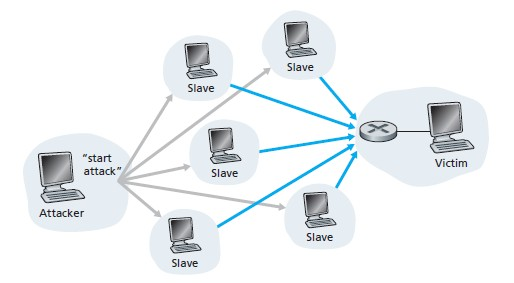
\includegraphics[width=0.95\linewidth]{cap21/ddos.png}
\end{minipage}\hfill
\begin{minipage}{0.52\linewidth}
Ci sono tre tipi di attacchi DoS:
\begin{enumerate}
  \item \textbf{Attacco a una vulnerabilità}: si inviano messaggi costruiti ad arte a un'applicazione o a un sistema operativo vulnerabile
        per bloccarlo o farlo andare in crash.
  \item \textbf{Bandwidth flooding}: si inonda l'host bersaglio di pacchetti, impedendo a quelli legittimi di raggiungerlo.
  \item \textbf{Connection flooding}: si aprono moltissime connessioni TCP, mezze aperte o complete, verso il bersaglio, che smette di
        accettare connessioni legittime (per esempio il \emph{SYN flood}).
\end{enumerate}
\end{minipage}
\caption{Un DDoS (\emph{Distributed DoS}): l'attaccante comanda una botnet di zombie che attaccano la vittima tutti insieme.}
\end{figure}

\info{Perché ``distribuito''}{
    Un solo attaccante ha banda limitata ed è facile da bloccare filtrando il suo indirizzo. Con migliaia di zombie sparsi per il mondo
    il traffico è enorme e proviene da indirizzi diversi, quindi è molto più difficile da distinguere da quello legittimo.
}

\subsection{Riflessione e amplificazione}

Migliaia di server DNS cominciano a mandarvi risposte a domande che non avete mai fatto. Chi ha inviato le domande? Un attaccante, con
il \textbf{vostro indirizzo come sorgente}. Una query UDP non richiede handshake, quindi nessuno la controlla: ogni server risponde
all'indirizzo che gli è stato dato.

\begin{itemize}
    \item \textbf{Riflessione}: il traffico vi raggiunge da server legittimi, quindi non c'è una botnet da rintracciare e niente di
          ovvio da bloccare.
    \item \textbf{Amplificazione}: una piccola query può portare una grande risposta, in media circa \textbf{55 volte} i byte per il
          DNS, oltre \textbf{500} per NTP. Attacchi costruiti così hanno raggiunto i terabit al secondo.
    \item La difesa sta alla sorgente, l'\textbf{egress filtering}: una rete scarta i pacchetti in uscita il cui indirizzo sorgente non
          è suo.
\end{itemize}

% ══════════════════════════════════════════════════════════════
\section{Il packet sniffing}
% ══════════════════════════════════════════════════════════════

\dfn{Packet sniffing}{
    Lo \textbf{sniffing} prevede un ricevitore \textbf{passivo} (lo \emph{sniffer}) che registra una copia dei pacchetti interessanti di un
    host bersaglio, cercando di rubare informazioni sensibili (\emph{eavesdropping}, origliare).
}

\begin{itemize}
    \item Gli sniffer si possono usare in qualunque rete \textbf{broadcast} (cablata o senza fili), semplicemente tenendo i frame
          destinati ad altri invece di scartarli.
    \item Uno switch rende la cosa più difficile, non impossibile: abbiamo visto come avvelenarne la tabella. Oppure un malware su un
          router copia tutto ciò che inoltra.
    \item Poiché gli sniffer sono \textbf{passivi} (non immettono traffico nella rete), sono \textbf{difficilissimi da rilevare}.
    \item Anche il traffico cifrato dice a uno sniffer \textbf{chi parla con chi, e quando}: ci torneremo parlando di anonimato.
    \item Ciò che deve restare privato va \textbf{cifrato}: è l'unica difesa che non dipende dal percorso.
\end{itemize}

\subsection{Uno sniffer che usate già}

Lo stesso Wireshark usato finora, nella sua versione da terminale, filtrato sulla connessione di controllo di FTP:

\begin{lstlisting}[language=bash]
$ sudo tshark -i enp3s0 -f 'tcp port 21' -Y ftp
  4 0.000000 192.168.1.17 -> 192.168.1.23 FTP 86 Response: 220 (vsFTPd 3.0.5)
  6 3.210114 192.168.1.23 -> 192.168.1.17 FTP 80 Request: USER ftpuser
  8 3.210706 192.168.1.17 -> 192.168.1.23 FTP 100 Response: 331 Please specify the password.
 10 6.041237 192.168.1.23 -> 192.168.1.17 FTP 81 Request: PASS reti2026
 12 6.088015 192.168.1.17 -> 192.168.1.23 FTP 89 Response: 230 Login successful.
\end{lstlisting}

\begin{itemize}
    \item Nome utente e password, \textbf{in chiaro}. E non è stato inviato nulla a nessuno: la cattura è silenziosa, e nessuno dei due
          estremi può accorgersene.
    \item Qui abbiamo intercettato il nostro traffico; su un mezzo condiviso, o con uno switch avvelenato, sarebbe quello di chiunque.
    \item Accedendo con FTPS o SSH la stessa cattura mostra solo record cifrati: è ciò che compra il gemello sicuro.
\end{itemize}

% ══════════════════════════════════════════════════════════════
\section{L'IP spoofing}
% ══════════════════════════════════════════════════════════════

\dfn{IP spoofing}{
    L'\textbf{IP spoofing} è la tecnica con cui un host malevolo immette nella rete pacchetti con \textbf{indirizzo sorgente falso}
    (contraffatto).
}

\begin{itemize}
    \item Con un'applicazione che si fida di certi indirizzi, permette all'attaccante di agire come un utente fidato.
    \item In un DoS, sorgenti falsificate sono molto più difficili da filtrare degli indirizzi di una botnet.
    \item È \textbf{facile} dovunque il protocollo non controlli: un frame Ethernet, un datagramma UDP, una risposta ARP, una risposta
          DNS.
    \item È \textbf{difficile} in TCP: un segmento falsificato richiede il numero di sequenza scelto dall'altra parte. È per questo che
          i numeri iniziali sono casuali.
    \item Le difese sono l'\textbf{integrità dei messaggi} e l'\textbf{autenticazione degli estremi}: è stato modificato, e chi l'ha
          inviato davvero?
\end{itemize}

% ══════════════════════════════════════════════════════════════
\section{Il man in the middle}
% ══════════════════════════════════════════════════════════════

\begin{itemize}
    \item Trudy si mette tra due host: ogni messaggio di ciascuna parte passa da lei.
    \item Finge di essere Bob con Alice e Alice con Bob, e ciascuno crede di parlare con l'altro.
    \item Può leggere, cambiare, ritardare o scartare qualsiasi cosa. Abbiamo visto un modo per arrivarci: avvelenare ARP con
          l'indirizzo del gateway.
    \item La cifratura da sola non li salva: se le chiavi sono state concordate con Trudy, lei decifra, legge e ricifra.
\end{itemize}

\begin{figure}[H]
\centering
\begin{tikzpicture}[every node/.style={font=\footnotesize\sffamily}]
  \node (a) at (0,0) {\icon[1cm]{pc}}; \node[below=-2pt of a] {A};
  \node (b) at (9,0) {\icon[1.1cm]{laptop}}; \node[below=-2pt of b] {B};
  \node[draw, fill=netred!20, rounded corners, minimum width=1.4cm, minimum height=0.8cm] (t) at (4.5,-1.2) {T (Trudy)};
  \draw[msg, netred, thick] (a) -- node[above, sloped] {``sono B''} (t);
  \draw[msg, netred, thick] (t) -- node[above, sloped] {``sono A''} (b);
  \draw[dashed, black!40, thick] (a) -- node[above] {A e B credono di parlare direttamente} (b);
\end{tikzpicture}
\caption{L'attacco man-in-the-middle: T finge di essere B con A e di essere A con B, intercettando i messaggi (spesso aiutandosi con lo spoofing).}
\end{figure}

% ══════════════════════════════════════════════════════════════
\section{Le proprietà di una comunicazione sicura}
% ══════════════════════════════════════════════════════════════

Visti i tipi di attacco, possiamo definire le proprietà che una comunicazione sicura dovrebbe garantire.

\dfn{Le quattro proprietà}{
    \begin{itemize}
      \item \textbf{Confidenzialità}: solo il mittente e il destinatario previsto devono poter capire il contenuto del messaggio
            (contro lo \emph{sniffing}).
      \item \textbf{Integrità del messaggio}: il contenuto non deve essere alterato, né in modo malevolo né per errore.
      \item \textbf{Autenticazione degli estremi} (\emph{end-point authentication}): mittente e destinatario devono poter confermare
            l'identità dell'altra parte (contro lo \emph{spoofing}).
      \item \textbf{Sicurezza operativa}: gli intrusi vengono tenuti fuori dalla rete (contro worm e intrusioni).
    \end{itemize}
}

Le prime tre sono costruite \textbf{dentro i protocolli}, e tutte e tre poggiano sulla crittografia. La quarta sta al \textbf{bordo}
della rete di un'organizzazione: firewall e sistemi di rilevazione delle intrusioni. Il Tanenbaum aggiunge la \textbf{disponibilità},
la proprietà che un denial of service attacca.

\begin{table}[H]
\centering
\begin{tabular}{lll}
\toprule
\textbf{Attacco} & \textbf{Proprietà violata} & \textbf{Contromisura} \\
\midrule
Sniffing & confidenzialità & crittografia \\
Alterazione dei messaggi & integrità & hash crittografici, MAC \\
Spoofing, replay & autenticazione & nonce, certificati \\
DoS, intrusioni, malware & sicurezza operativa & firewall, IDS \\
\bottomrule
\end{tabular}
\caption{Attacchi, proprietà e contromisure.}
\end{table}

% ══════════════════════════════════════════════════════════════
\section{Introduzione alla crittografia}
% ══════════════════════════════════════════════════════════════

\dfn{Crittografia}{
    Una tecnica \textbf{crittografica} permette a un mittente di \textbf{camuffare i dati} in modo che siano incomprensibili per un intruso:
    l'intruso non deve ricavare alcuna informazione dai dati intercettati, mentre il destinatario deve poter recuperare i dati originali.
    \begin{itemize}
      \item Nella sua forma iniziale il messaggio si chiama \textbf{testo in chiaro} (\emph{plaintext} o \emph{cleartext}) ed è leggibile da tutti.
      \item Prima di immetterlo nel canale, il mittente usa un \textbf{algoritmo di cifratura} che lo trasforma in una forma illeggibile, il
            \textbf{testo cifrato} (\emph{ciphertext}), che va \textbf{decifrato} alla ricezione.
    \end{itemize}
}

\begin{figure}[H]
    \centering
    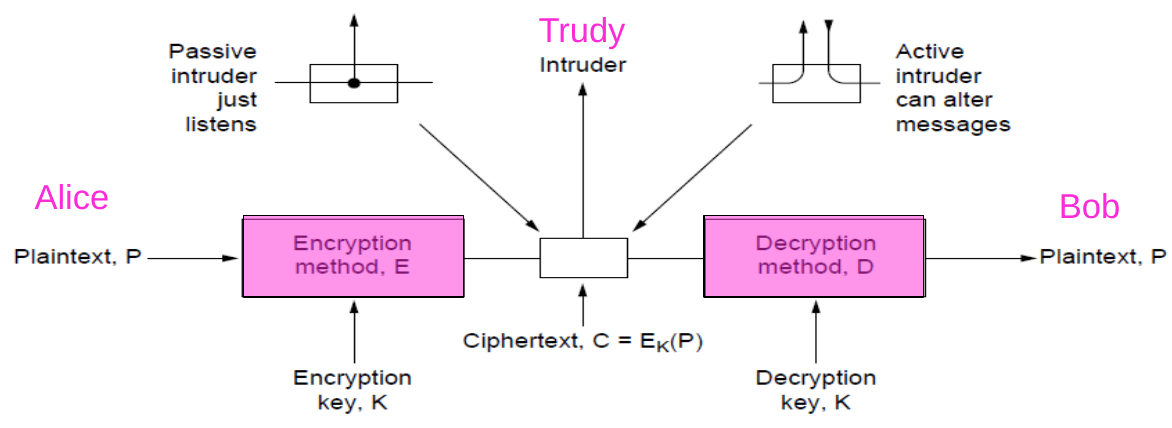
\includegraphics[width=0.72\linewidth]{cap21/modello_intruso.png}
    \caption{Il modello di cifratura (da Tanenbaum): Alice cifra con la chiave $K_E$, Bob decifra con $K_D$; Trudy può ascoltare passivamente o intervenire attivamente.}
\end{figure}

Un intruso \textbf{passivo} si limita ad ascoltare, ed è esattamente ciò che la cifratura sconfigge. Un intruso \textbf{attivo} può
anche alterare, iniettare e ripetere messaggi: contro di lui la cifratura da sola non basta.

Con la notazione del Tanenbaum:

\begin{itemize}
    \item $K$ è la \textbf{chiave}, $P$ il messaggio in chiaro (\emph{plaintext}), $C$ il messaggio cifrato (\emph{ciphertext});
    \item la cifratura con chiave $K$ si scrive $E_K(P) = C$ e la decifratura $D_K(C) = P$, quindi $D_K(E_K(P)) = P$.
\end{itemize}

Nella notazione del Kurose, usata nelle slide, Alice cifra $m$ con la propria chiave $K_A$ e invia $K_A(m)$; Bob decifra con la propria
chiave $K_B$: $K_B(K_A(m)) = m$.

\subsection{Le chiavi e il principio di Kerckhoffs}

Nei sistemi crittografici moderni, compresi quelli di Internet, la tecnica di cifratura è \textbf{nota e standard per tutti} (anche per
l'intruso). La parte sconosciuta sono le \textbf{chiavi di cifratura e decifratura}.

\dfn{Chiave}{
    Una \textbf{chiave} è una stringa alfanumerica che va fornita all'algoritmo di cifratura o decifratura per cifrare o decifrare i messaggi.
    Le chiavi di cifratura e decifratura possono essere \textbf{identiche} (crittografia \emph{simmetrica}) o \textbf{diverse}
    (\emph{asimmetrica}).
}

\dfn{Principio di Kerckhoffs}{
    \textbf{Tutti gli algoritmi devono essere pubblici; solo le chiavi sono segrete.} La ``sicurezza per oscurità'' (\emph{security by
    obscurity}), cioè tenere segreto l'algoritmo, non funziona mai: prima o poi l'algoritmo trapela, e allora tutto è esposto.
}

\begin{itemize}
    \item Un algoritmo richiede anni per essere progettato e diffuso; una chiave si cambia in un secondo, tutte le volte che serve.
    \item Un algoritmo pubblicato viene attaccato gratis da ogni crittografo: se resiste per anni, probabilmente è solido.
    \item Il segreto sta quindi tutto nella chiave, e la sua \textbf{lunghezza} conta: $n$ bit sono $2^n$ chiavi da provare, e ogni bit in
          più raddoppia il lavoro.
\end{itemize}

\subsection{I problemi della crittoanalisi}

Chi cerca di ``rompere'' un cifrario (il \emph{crittoanalista}) può trovarsi in tre situazioni, ciascuna più favorevole della
precedente:

\begin{table}[H]
\centering
\begin{tabular}{lll}
\toprule
\textbf{Attacco} & \textbf{Che cosa ha Trudy} & \textbf{Per esempio} \\
\midrule
solo testo cifrato & testo cifrato intercettato, nient'altro & le frequenze delle lettere \\
testo in chiaro noto & alcune coppie di testo in chiaro e cifrato & ``bob'' e ``alice'' ci sono di sicuro \\
testo in chiaro scelto & il cifrato di testi scelti da lei & Alice invia un testo scelto da Trudy \\
\bottomrule
\end{tabular}
\caption{Che cosa ha a disposizione il crittoanalista.}
\end{table}

Il testo in chiaro noto è il caso \textbf{normale}, non sfortuna: molte macchine cominciano ogni sessione con le stesse parole, come
\texttt{login:}. Un cifrario si giudica quindi sull'attacco più forte: deve resistere anche al testo in chiaro scelto.

\subsection{Cifrari per sostituzione}

\dfn{Cifrario per sostituzione}{
    In un cifrario per \textbf{sostituzione} ogni simbolo viene sostituito con un altro. La chiave è la \textbf{corrispondenza tra simboli}.
}

Il più antico è il \textbf{cifrario di Cesare}: ogni lettera viene sostituita da quella $k$ posti più avanti; con $k = 3$,
\texttt{attacco} diventa \texttt{dwwdffr}. Ci sono solo 25 chiavi da provare. Il cifrario \textbf{monoalfabetico} permette invece
qualsiasi corrispondenza, purché biunivoca: la chiave è l'intera seconda riga.

\begin{center}
\begin{tabular}{rl}
testo in chiaro: & \texttt{a b c d e f g h i j k l m n o p q r s t u v w x y z} \\
testo cifrato: & \texttt{Q W E R T Y U I O P A S D F G H J K L Z X C V B N M} \\
\end{tabular}
\end{center}

Con questa chiave \texttt{attacco} diventa \texttt{QZZQEEG}. Anche se le chiavi possibili sono $26! \approx 4\cdot 10^{26}$, per l'alfabeto
latino (e altri) questi cifrari sono \textbf{facilmente attaccabili}: provarle tutte è senza speranza, ma il cifrario conserva le
\textbf{regolarità statistiche} della lingua, e una pagina di testo cifrato basta. In inglese \emph{e} e \emph{t} sono il 13\% e il 9\%
delle lettere; in italiano le più frequenti sono e, a, i, o, le doppie sono frequenti e certe coppie di lettere sono comunissime. Si
contano le lettere, si accoppiano le più frequenti, poi le coppie frequenti: il cifrario ha solo valore didattico, e non si usa mai.

\subsection{Cifrari per trasposizione}

\dfn{Cifrario per trasposizione}{
    In un cifrario per \textbf{trasposizione} i simboli \textbf{non cambiano}, ma vengono \textbf{riordinati}. Nel cifrario a trasposizione per
    colonne la chiave è una parola senza lettere ripetute: le sue lettere, in ordine alfabetico, danno l'ordine con cui leggere le colonne.
}

\begin{figure}[H]
    \centering
    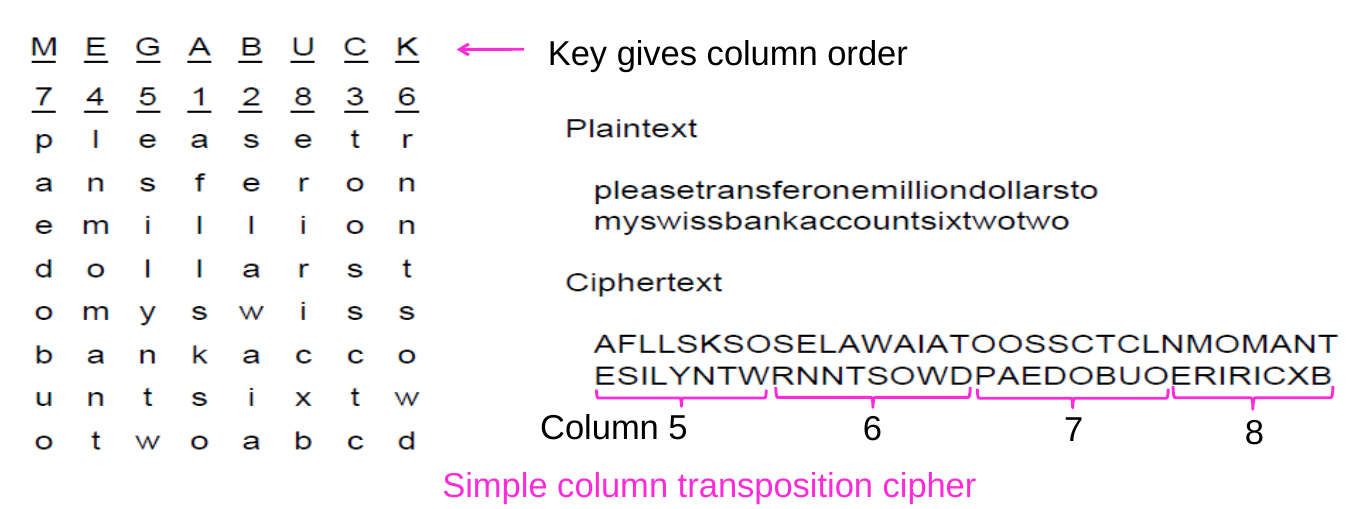
\includegraphics[width=0.55\linewidth]{cap21/trasposizione.png}
    \caption{Trasposizione per colonne con chiave MEGABUCK (da Tanenbaum): il testo si scrive per righe e si legge colonna per colonna, nell'ordine indicato dai numeri.}
\end{figure}

\begin{itemize}
    \item La chiave fissa l'ordine delle colonne, alfabetico: prima la A. La colonna 1 dà \texttt{AFLLSKSO}, e il testo cifrato completo
          è \texttt{AFLLSKSOSELAWAIATOOSSCTCLNMOMANTESILYNTWRNNTSOWDPAEDOBUOERIRICXB}.
    \item Ogni lettera continua a rappresentare sé stessa, quindi le frequenze sono quelle della lingua: questo da solo tradisce una
          trasposizione.
    \item Una frase indovinata, come \texttt{milliondollars}, rivela poi il numero di colonne, e il resto segue.
\end{itemize}

% ══════════════════════════════════════════════════════════════
\section{La crittografia simmetrica}
% ══════════════════════════════════════════════════════════════

\dfn{Crittografia simmetrica}{
    Nella crittografia \textbf{simmetrica} c'è \textbf{una sola chiave}, usata sia per cifrare sia per decifrare.
    \begin{itemize}
      \item \textbf{Cifratura}: il testo in chiaro, insieme alla chiave, viene passato all'algoritmo di cifratura, che genera un testo cifrato
            che può viaggiare in rete in sicurezza.
      \item \textbf{Decifratura}: il testo cifrato, insieme alla chiave, viene passato all'algoritmo di decifratura, che ricrea il testo in chiaro.
    \end{itemize}
}

\begin{figure}[H]
\centering
\begin{tikzpicture}[every node/.style={font=\footnotesize\sffamily}]
  \node[draw, fill=white, rounded corners] (p1) at (0,0) {testo in chiaro};
  \node[draw, fill=netred!20, minimum width=2cm, minimum height=0.8cm] (e) at (3,0) {cifratura};
  \node[draw, fill=lphy!60, rounded corners] (c) at (6.5,0) {testo cifrato};
  \node[draw, fill=netgreen!20, minimum width=2cm, minimum height=0.8cm] (d) at (10,0) {decifratura};
  \node[draw, fill=white, rounded corners] (p2) at (13,0) {testo in chiaro};
  \draw[msg] (p1) -- (e); \draw[msg] (e) -- (c); \draw[msg] (c) -- node[above, text=netred] {canale} (d); \draw[msg] (d) -- (p2);
  \node (k1) at (3,1.3) {chiave $K$};
  \node (k2) at (10,1.3) {stessa chiave $K$};
  \draw[msg] (k1) -- (e); \draw[msg] (k2) -- (d);
  \node[draw, fill=netred!15, rounded corners] (t) at (6.5,-1.3) {intruso};
  \draw[msg, dashed, netred] (c) -- node[right] {sniffing: vede solo il cifrato} (t);
\end{tikzpicture}
\caption{Crittografia simmetrica: la stessa chiave serve a cifrare e a decifrare.}
\end{figure}

È così che la crittografia ha funzionato per duemila anni, e porta ancora quasi tutti i dati cifrati di oggi.

\subsection{Il one-time pad}

\dfn{One-time pad}{
    Il \textbf{one-time pad} è un cifrario \textbf{inviolabile}: si sceglie come chiave (il \emph{pad}) una stringa di bit
    \textbf{casuale}, lunga quanto il messaggio, e si cifra facendo lo XOR bit a bit: $C = P \oplus K$. Per decifrare si rifà lo XOR con lo
    stesso pad: $C \oplus K = P \oplus K \oplus K = P$.
}

\begin{esempio}{Cifrare e decifrare con lo XOR}
Con $P = \texttt{0111}$ e $K = \texttt{1101}$:
\begin{center}
\begin{tabular}{lcl}
cifratura & $P \oplus K$ & $= \texttt{0111} \oplus \texttt{1101} = \texttt{1010} = C$ \\
decifratura & $C \oplus K$ & $= \texttt{1010} \oplus \texttt{1101} = \texttt{0111} = P$ \\
\end{tabular}
\end{center}
\end{esempio}

\begin{figure}[H]
    \centering
    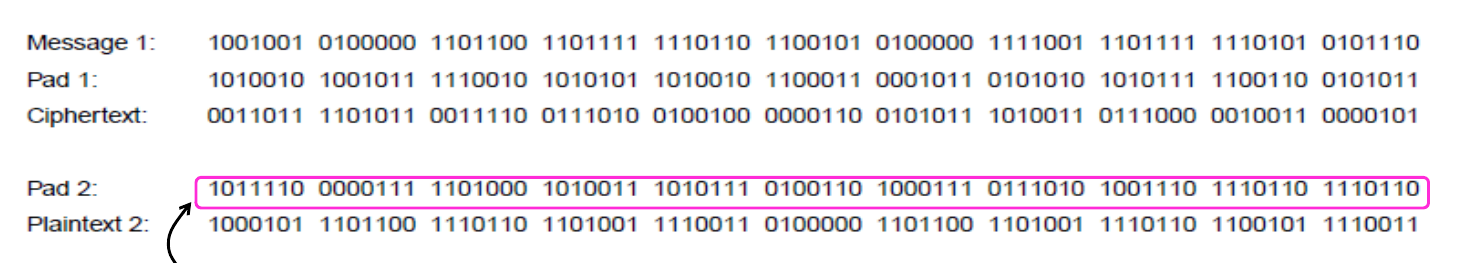
\includegraphics[width=0.82\linewidth]{cap21/one_time_pad.png}
    \caption{Con il one-time pad, dallo stesso testo cifrato si ottengono testi in chiaro diversi usando pad diversi (da Tanenbaum): senza il pad, ogni messaggio della stessa lunghezza è ugualmente probabile.}
\end{figure}

Il one-time pad introduce una grande quantità di ridondanza e impedisce che qualsiasi informazione del testo in chiaro $P$ si rifletta nel
testo cifrato $C$. Ha però problemi pratici:

\begin{enumerate}
    \item \textbf{condivisione del pad}: il pad (la chiave) va distribuito in sicurezza;
    \item \textbf{errori di sincronizzazione}: se il messaggio ha uno spostamento (un bit perso), la decifratura fallisce da lì in poi;
    \item il punto vero: il pad ha la \textbf{stessa dimensione del messaggio}. Se si ha un modo sicuro di trasmettere il pad, tanto vale
          trasmettere direttamente il messaggio (salvo casi particolari, come uno scambio di persona del pad su un supporto fisico).
\end{enumerate}

\warning{One-time vuol dire una volta sola}{
    Un pad \textbf{non deve mai essere usato più di una volta}: se due messaggi sono cifrati con lo stesso pad, Trudy fa lo XOR dei due
    cifrati, $C_1 \oplus C_2 = P_1 \oplus P_2$: il pad si annulla, e le statistiche della lingua fanno il resto.
}

Il one-time pad si usa solo dove il pad può viaggiare a mano, su un disco, prima che venga inviato qualsiasi messaggio. È lo
\emph{scrambling} del livello fisico, ancora una volta, ma con una sequenza davvero casuale e segreta. I \textbf{cifrari a flusso}
(\emph{stream cipher}) generano un lungo flusso di chiave da una chiave corta: sono pratici, e legati alla stessa regola, non
riusarlo mai.

\subsection{Due principi fondamentali}

\dfn{I due principi della crittografia}{
    \begin{enumerate}
      \item \textbf{Ridondanza}: ogni messaggio cifrato deve contenere una qualche forma di ridondanza. Altrimenti un attaccante potrebbe inviare
            un messaggio cifrato \textbf{a caso}, che dopo la decifratura verrebbe accettato come valido.
      \item \textbf{Freschezza}: serve un meccanismo per prevenire la \textbf{ripetizione} di vecchi messaggi (\emph{replay attack}).
    \end{enumerate}
}

\begin{esempio}{Ridondanza e freschezza in pratica}
\begin{itemize}
    \item \textbf{Ridondanza}: un ordine è fatto di 3 byte cifrati, quantità e prodotto. Trudy non ha la chiave e invia byte a caso. Bob li
          decifra, e quasi ogni stringa di 3 byte è un ordine valido: spedisce 837 altalene a un cliente vero. Se invece ogni messaggio
          contiene un campo di controllo (per esempio $h = H(m)$, così che si invia $E_K(m, h)$), Bob decifra, ricalcola $H(m)$ e verifica
          la corrispondenza: bit casuali la superano solo per caso, con probabilità trascurabile. La ridondanza aiuta però anche un
          crittoanalista passivo a riconoscere un tentativo giusto: quindi mai una sequenza di zeri, sempre qualcosa come un hash.
    \item \textbf{Freschezza}: Trudy registra un messaggio cifrato valido da Alice a Bob (per esempio ``paga 100 euro a T'') e lo rimanda
          il giorno dopo. Nessun controllo fallisce: il messaggio è autentico, quindi si decifra e si verifica perfettamente, ed è un
          \textbf{replay attack}. Si risolve con un \textbf{timestamp} dentro il messaggio cifrato (ridondanza sul tempo, non sul
          contenuto): Bob rifiuta tutto ciò che è più vecchio, diciamo, di 60 secondi, e ricorda ciò che ha visto in quella finestra.
          Oppure con un \textbf{nonce}, un numero usato una sola volta: freschezza senza orologi sincronizzati.
\end{itemize}
\end{esempio}

\subsection{I cifrari a blocchi}

\begin{minipage}{0.28\linewidth}
\centering
\begin{tabular}{cc}
\toprule
\textbf{in} & \textbf{out} \\
\midrule
\texttt{000} & \texttt{110} \\
\texttt{001} & \texttt{111} \\
\texttt{010} & \texttt{101} \\
\texttt{011} & \texttt{100} \\
\texttt{100} & \texttt{011} \\
\texttt{101} & \texttt{010} \\
\texttt{110} & \texttt{000} \\
\texttt{111} & \texttt{001} \\
\bottomrule
\end{tabular}
\end{minipage}\hfill
\begin{minipage}{0.68\linewidth}
\begin{itemize}
    \item Il messaggio viene tagliato in blocchi di $k$ bit, e ogni blocco viene associato in modo biunivoco a un blocco di $k$ bit di
          testo cifrato.
    \item Con $k = 3$ la tabella è la chiave: \texttt{010110001111} diventa \texttt{101000111001}.
    \item Una corrispondenza è una permutazione dei $2^k$ ingressi: qui $8! = 40\,320$ chiavi, $(2^k)!$ in generale.
    \item Con $k = 64$ la tabella avrebbe $2^{64}$ righe. I cifrari reali quindi la \textbf{calcolano}: piccole tabelle e un rimescolatore
          di bit, ripetuti per diversi \textbf{round}, che fanno sì che ogni bit d'ingresso influenzi quasi ogni bit d'uscita.
\end{itemize}
\end{minipage}


\subsection{DES e AES}

\dfn{DES (Data Encryption Standard)}{
    Il \textbf{DES} è lo standard statunitense del 1977:
    \begin{itemize}
      \item il testo in chiaro viene cifrato a \textbf{blocchi di 64 bit};
      \item la cifratura avviene in \textbf{19 stadi}, di cui 16 round;
      \item usa una chiave da \textbf{56 bit}: troppo corta fin dall'inizio, è stata violata per forza bruta da tempo.
    \end{itemize}
}

\begin{figure}[H]
    \centering
    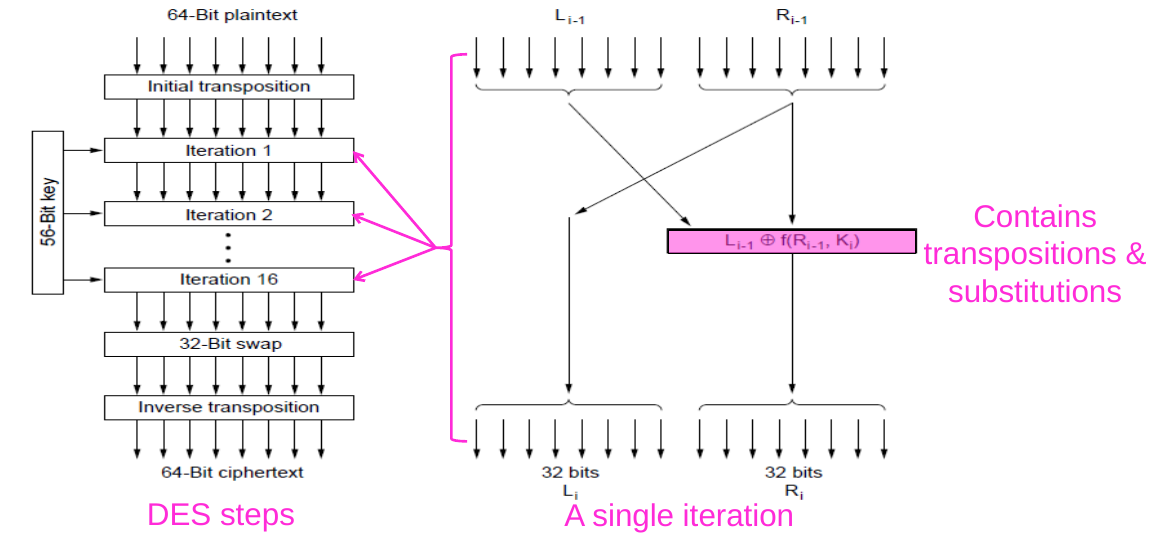
\includegraphics[width=0.62\linewidth]{cap21/des.png}
    \caption{La struttura del DES (da Tanenbaum): a sinistra i 19 stadi, a destra una singola iterazione.}
\end{figure}

\begin{itemize}
    \item Il primo e l'ultimo stadio sono \textbf{trasposizioni} (una inversa dell'altra); il diciottesimo scambia i due blocchi da 32 bit.
    \item Nei 16 stadi intermedi, detti iterazioni: i 32 bit di sinistra dell'uscita sono i 32 bit di destra dell'ingresso ($L_i = R_{i-1}$);
          quelli di destra sono $L_{i-1} \oplus f(R_{i-1}, K_i)$, dove la funzione $f$ \textbf{espande}, fa lo \textbf{XOR con la chiave}
          dell'iterazione $K_i$ e applica \textbf{sostituzioni} e \textbf{trasposizioni}.
    \item La chiave $K_i$ è diversa per ogni iterazione (una diversa selezione dei bit della chiave principale).
    \item La decifratura è lo stesso circuito, con le chiavi in ordine inverso.
\end{itemize}

\begin{itemize}
    \item \textbf{Triple DES}: cifra, decifra, cifra con le chiavi $K_1, K_2, K_1$; con $K_1 = K_2$ parla con il DES semplice. Oggi
          obsoleto.
    \item \textbf{AES} (\emph{Advanced Encryption Standard}): scelto nel 2001 con un concorso aperto, quindici proposte pubbliche attaccate
          in pubblico per anni prima della scelta. Blocchi da 128 bit, chiavi da 128, 192 o 256 bit, da 10 a 14 round, tutto su byte
          interi: veloce in software, e integrato nelle CPU.
    \item Una macchina che provasse tutte le $2^{56}$ chiavi DES in un secondo impiegherebbe circa \textbf{149 mila miliardi di anni}
          per l'AES-128.
\end{itemize}

\subsection{Le modalità di cifratura: ECB e CBC}

\warning{Stesso blocco in ingresso, stesso blocco in uscita}{
    Due blocchi di testo in chiaro sono identici. Che cosa vede Trudy? Due blocchi di testo cifrato identici: con la tabella del cifrario
    a blocchi, \texttt{010 010 010} viene inviato come \texttt{101 101 101}. Cifrare blocco per blocco è la modalità \textbf{ECB}
    (\emph{Electronic Code Book}), e un cifrario a blocchi usato così è un \textbf{cifrario monoalfabetico con lettere da 128 bit}.
    \begin{itemize}
      \item Le regolarità del testo in chiaro traspaiono nel cifrato: un \texttt{HTTP/1.1} ripetuto rivela la struttura del protocollo.
      \item Un Trudy attivo fa di peggio. Un file di stipendi è cifrato record per record, e ogni premio è un blocco: Leslie copia il
            blocco che contiene il premio di un collega sopra il proprio. Senza la chiave, e il risultato si decifra perfettamente.
    \end{itemize}
}

\Needspace{9\baselineskip}
\dfn{CBC (Cipher Block Chaining)}{
    Il \textbf{CBC} è una modalità di cifratura molto usata che \textbf{concatena} i blocchi con lo XOR:
    $$C_0 = E_K(P_0 \oplus IV), \qquad C_i = E_K(P_i \oplus C_{i-1})$$
    dove $IV$ è un \textbf{vettore di inizializzazione} casuale, diverso per ogni messaggio. Così lo stesso blocco in chiaro produce blocchi
    cifrati diversi a seconda di tutto ciò che lo precede.
}

\begin{figure}[H]
    \centering
    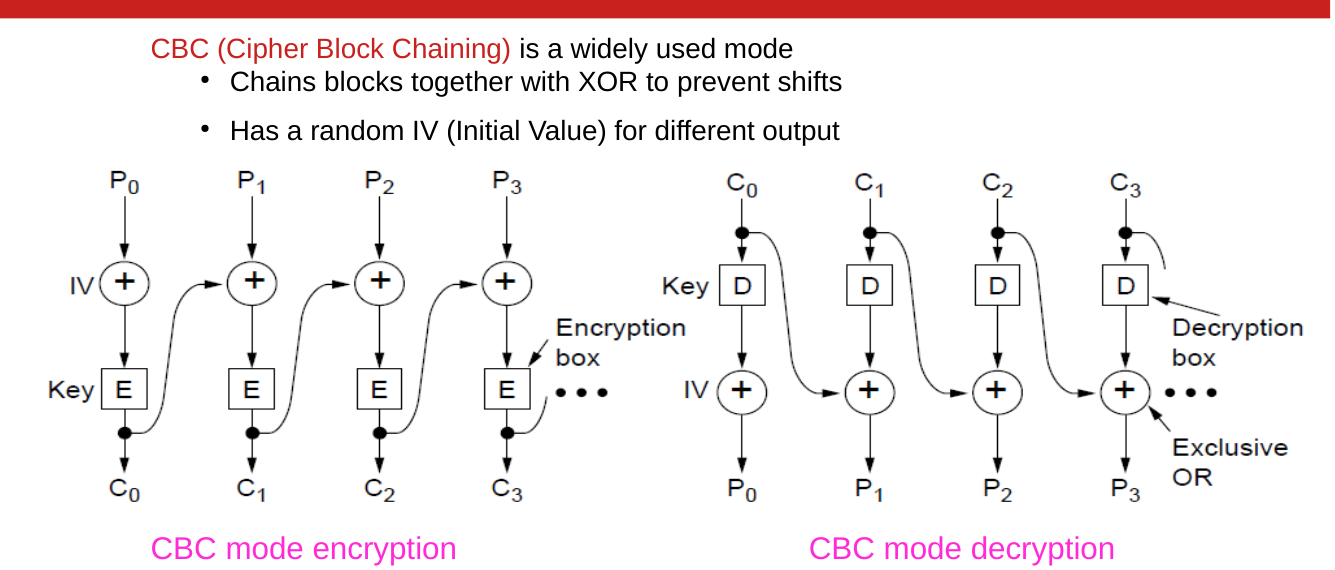
\includegraphics[width=0.75\linewidth]{cap21/cbc.png}
    \caption{CBC: cifratura (a sinistra) e decifratura (a destra), $P_i = D_K(C_i) \oplus C_{i-1}$.}
\end{figure}

\begin{esempio}{Tre blocchi uguali, tre cifrati diversi}
Con la tabella a 3 bit dei cifrari a blocchi, testo in chiaro \texttt{010 010 010} e IV \texttt{001}:
\begin{center}
\begin{tabular}{l}
$c(1) = K_S(\texttt{010} \oplus \texttt{001}) = K_S(\texttt{011}) = \texttt{100}$ \\
$c(2) = K_S(\texttt{010} \oplus \texttt{100}) = K_S(\texttt{110}) = \texttt{000}$ \\
$c(3) = K_S(\texttt{010} \oplus \texttt{000}) = K_S(\texttt{010}) = \texttt{101}$ \\
\end{tabular}
\end{center}
\end{esempio}

\begin{itemize}
    \item L'IV viaggia in chiaro: senza la chiave non serve a Trudy. Bob decifra $c(i)$ con $K_S$ e fa lo XOR del risultato con
          $c(i-1)$, che ha già.
    \item Il costo è un blocco in più, l'IV, che ogni protocollo che usa il CBC deve portare: lo ritroveremo dentro TLS, fino alla
          versione 1.2.
    \item Un blocco incollato da un'altra parte rovina due blocchi: Leslie viene scoperta.
\end{itemize}

% ══════════════════════════════════════════════════════════════
\section{Lo scambio delle chiavi}
% ══════════════════════════════════════════════════════════════


\warning{Come ci si scambia la chiave?}{
    Il problema della crittografia simmetrica (a chiave singola) è che la chiave segreta deve essere \textbf{comunicata} (\emph{key
    exchange problem}).
    \begin{itemize}
      \item Gli host possono usare un \textbf{canale sicuro} per scambiarsi la chiave.
      \item Gli host possono usare un \textbf{protocollo} che permetta loro di ``convergere'' su una chiave condivisa.
    \end{itemize}
    Se due parti non riescono a stabilire in modo sicuro la chiave iniziale, non potranno comunicare in sicurezza: un terzo che abbia
    intercettato la chiave durante lo scambio potrà leggere tutti i messaggi. Inoltre, con $N$ utenti che vogliono parlare a coppie servono
    $\frac{N(N-1)}{2}$ chiavi, una per ogni coppia (dell'ordine di $N^2$).
}

\subsection{Lo scambio di chiavi Diffie-Hellman}

\dfn{Diffie-Hellman}{
    Il protocollo \textbf{Diffie-Hellman} permette a due parti di stabilire un \textbf{segreto condiviso} su un canale pubblico.
    \begin{enumerate}
      \item Alice e Bob concordano in pubblico un primo grande $p$ e un numero $g$. Anche Trudy li conosce.
      \item Alice sceglie un segreto $S_A$ e invia $T_A = g^{S_A} \bmod p$; Bob sceglie $S_B$ e invia $T_B = g^{S_B} \bmod p$.
      \item Alice calcola $T_B^{S_A} \bmod p$, Bob $T_A^{S_B} \bmod p$: entrambi valgono $g^{S_A S_B} \bmod p$, la stessa chiave.
    \end{enumerate}
    Trudy ha $p$, $g$, $T_A$ e $T_B$. Per ricavare $S_A$ da $T_A$ le serve un \textbf{logaritmo discreto}, e non se ne conosce un metodo
    veloce.
}

\begin{esempio}{Diffie-Hellman con numeri piccoli}
$p = 47$, $g = 3$, $S_A = 8$, $S_B = 10$. Alice invia $3^8 \bmod 47 = 28$, Bob invia $3^{10} \bmod 47 = 17$. Alice calcola
$17^8 \bmod 47 = 4$, Bob $28^{10} \bmod 47 = 4$. La chiave non ha mai attraversato la rete.
\end{esempio}

\begin{figure}[H]
    \centering
    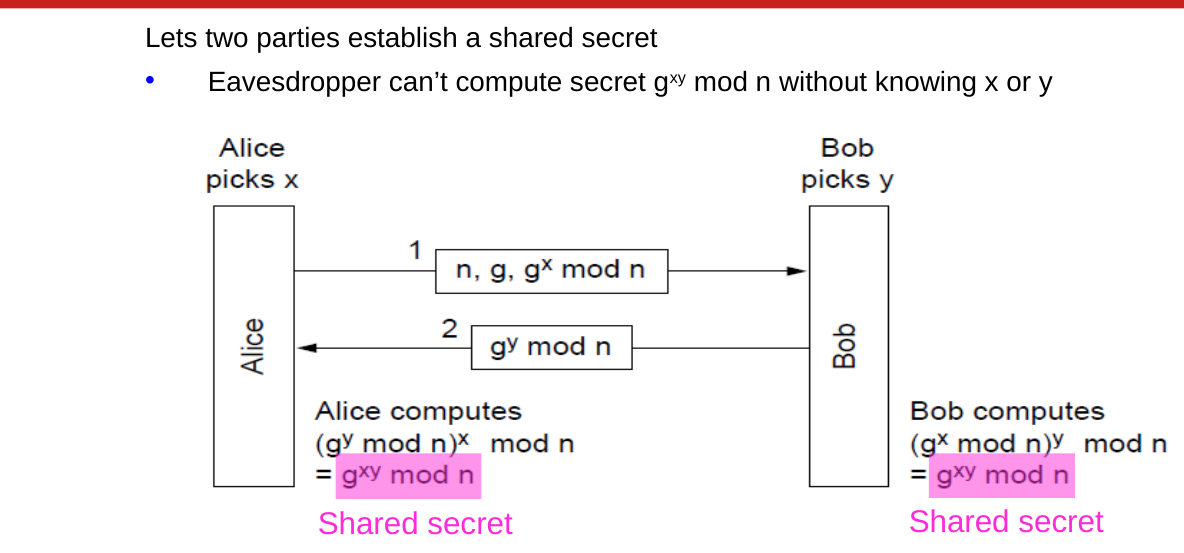
\includegraphics[width=0.52\linewidth]{cap21/dh.png}
    \caption{Lo scambio di chiavi Diffie-Hellman.}
\end{figure}

\warning{L'attacco man-in-the-middle a Diffie-Hellman}{
    Quando Bob riceve $T_A$, come sa che viene da Alice? \textbf{Non lo sa}. Trudy intercetta entrambi i valori e risponde a ciascuna parte
    con il proprio $T_T$: ci sono due chiavi, $g^{S_A S_T}$ e $g^{S_B S_T}$, e le ha entrambe. I messaggi di Alice si decifrano da Trudy,
    vengono letti, cambiati se vuole, e ricifrati per Bob; nessuno dei due vede niente di strano. Diffie-Hellman concorda una chiave, ma
    non dice nulla su \textbf{con chi}: serve un'autenticazione sopra, ed è il ruolo dei certificati.
    \begin{center}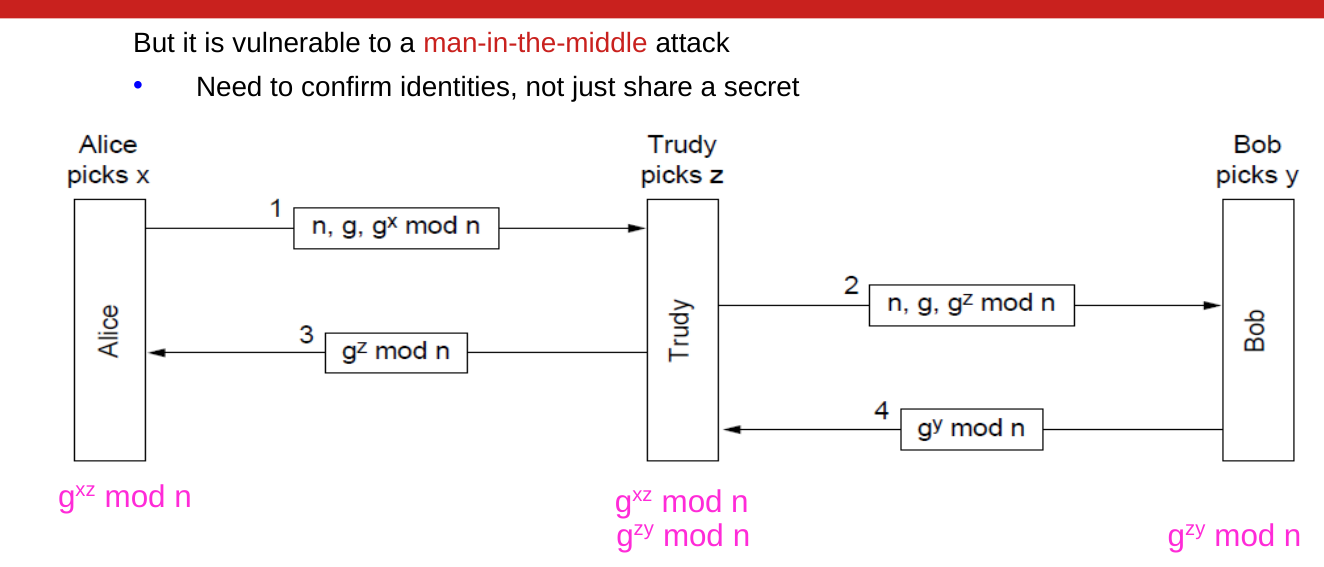
\includegraphics[width=0.55\linewidth]{cap21/dh_attacco.png}\end{center}
}

% ══════════════════════════════════════════════════════════════
\section{La crittografia asimmetrica}
% ══════════════════════════════════════════════════════════════

\dfn{Crittografia asimmetrica (a chiave pubblica)}{
    Nella crittografia \textbf{asimmetrica} ci sono \textbf{due chiavi} per ogni partecipante: una \textbf{pubblica} e una \textbf{privata}.
    \begin{itemize}
      \item Un messaggio cifrato con una delle due chiavi va decifrato con l'altra, e viceversa.
      \item La chiave pubblica può essere inviata su canali non sicuri o pubblicata; la chiave privata è disponibile \textbf{solo al proprietario}.
    \end{itemize}
}

\begin{figure}[H]
\centering
\begin{tikzpicture}[every node/.style={font=\footnotesize\sffamily}]
  \node[draw, fill=white, rounded corners] (p1) at (0,0) {testo in chiaro};
  \node[draw, fill=netred!20, minimum width=2cm, minimum height=0.8cm] (e) at (3,0) {cifratura};
  \node[draw, fill=lphy!60, rounded corners] (c) at (6.5,0) {testo cifrato};
  \node[draw, fill=netgreen!20, minimum width=2cm, minimum height=0.8cm] (d) at (10,0) {decifratura};
  \node[draw, fill=white, rounded corners] (p2) at (13,0) {testo in chiaro};
  \draw[msg] (p1) -- (e); \draw[msg] (e) -- (c); \draw[msg] (c) -- (d); \draw[msg] (d) -- (p2);
  \node (k1) at (3,1.3) {chiave \textbf{pubblica} di B};
  \node (k2) at (10,1.3) {chiave \textbf{privata} di B};
  \draw[msg] (k1) -- (e); \draw[msg] (k2) -- (d);
  \node[draw, fill=netred!15, rounded corners, text width=4.5cm, align=center] (t) at (6.5,-1.5) {l'intruso può conoscere la chiave pubblica, ma non può decifrare};
  \draw[msg, dashed, netred] (c) -- (t);
\end{tikzpicture}
\caption{A cifra con la chiave pubblica di B; solo B, con la propria chiave privata, può decifrare.}
\end{figure}

L'uso tipico: cifrare con la \textbf{chiave pubblica} del destinatario e decifrare con la sua \textbf{chiave privata}. Bob ha due chiavi:
una pubblica, $K_B^+$, per tutto il mondo, e una privata, $K_B^-$, che non lo lascia mai. Alice cifra con $K_B^+$, e solo $K_B^-$ la
disfa: $K_B^-(K_B^+(m)) = m$. Nessun segreto viene scambiato.

\begin{itemize}
    \item Se l'intruso intercetta la chiave pubblica, non riesce comunque a decifrare i messaggi.
    \item L'host A usa la chiave pubblica di B per cifrare messaggi che si possono leggere solo con la chiave privata di B, che è solo nelle mani di B.
    \item Con RSA le chiavi funzionano anche al contrario, $K_B^+(K_B^-(m)) = m$: è la base delle \textbf{firme digitali}.
    \item Ma chiunque può cifrare per Bob: il testo cifrato non dice nulla su \textbf{chi} l'ha inviato.
\end{itemize}

\info{Pro e contro rispetto alla crittografia simmetrica}{
    \begin{itemize}
      \item[\itick] La chiave privata \textbf{non va distribuita}; basta una coppia di chiavi per utente (invece di $N^2$ chiavi a coppie).
      \item[\icross] La sicurezza si basa su proprietà matematiche ed è molto \textbf{più lenta} (circa 1000 volte) della crittografia simmetrica.
    \end{itemize}
    Per questo la si usa soprattutto per \textbf{stabilire chiavi simmetriche di sessione}, con cui poi si cifrano i dati.
}

\dfn{Requisiti di un algoritmo a chiave pubblica}{
    \begin{enumerate}
      \item $D(E(P)) = P$ (correttezza);
      \item deve essere estremamente difficile ricavare la chiave privata da quella pubblica;
      \item $E$ non deve poter essere violato con un attacco a \textbf{testo in chiaro scelto}: l'intruso ha la chiave pubblica, quindi può cifrare
            tutti i testi in chiaro che vuole.
    \end{enumerate}
}

\Needspace{18\baselineskip}
\subsection{RSA}

\dfn{RSA}{
    L'\textbf{RSA} (Rivest, Shamir, Adleman) è l'algoritmo a chiave pubblica più diffuso. La sua sicurezza si basa sulla difficoltà di
    \textbf{fattorizzare numeri grandi}.
    \begin{itemize}
      \item \textbf{Generazione delle chiavi}: si scelgono due numeri primi grandi $p$ e $q$ (oggi il loro prodotto ha almeno 2048 bit); si
            calcolano $n = p \cdot q$ e $z = (p-1)(q-1)$; si sceglie $e < n$ senza fattori comuni con $z$; si trova $d$ tale che
            $e \cdot d \bmod z = 1$. La chiave \textbf{pubblica} è $K_B^+ = (n, e)$, quella \textbf{privata} è $K_B^- = (n, d)$.
      \item \textbf{Cifratura}: un messaggio è una sequenza di bit, quindi un numero $m < n$: $c = m^e \bmod n$.
      \item \textbf{Decifratura}: $m = c^d \bmod n$.
    \end{itemize}
    Da $n$ ed $e$ si ottiene $d$ solo fattorizzando $n$ in $p$ e $q$, e non se ne conosce un modo veloce.
}

\begin{esempio}{RSA con numeri piccoli (da Kurose)}
$p = 5$, $q = 7$: $n = 35$, $z = 24$; $e = 5$, e $d = 29$ perché $5 \cdot 29 - 1 = 144 = 6 \cdot 24$. Ogni lettera è il suo numero
nell'alfabeto, cifrato con $(35, 5)$ e decifrato con $(35, 29)$:
\begin{center}
\begin{tabular}{crrrr}
\toprule
 & $m$ & $m^e$ & $c$ & $c^d \bmod n$ \\
\midrule
l & 12 & 248\,832 & 17 & 12 \\
o & 15 & 759\,375 & 15 & 15 \\
v & 22 & 5\,153\,632 & 22 & 22 \\
e & 5 & 3125 & 10 & 5 \\
\bottomrule
\end{tabular}
\end{center}
\texttt{o} e \texttt{v} escono invariate: con numeri così piccoli RSA è solo un cifrario per sostituzione. Perché funziona: con
$n = pq$, $m^{ed} \bmod n = m^{ed \bmod z} \bmod n = m^1 = m$. La stessa identità letta al contrario dà $(m^d)^e = m$.
\end{esempio}

\subsection{Le chiavi di sessione}

\begin{itemize}
    \item RSA è lento: esponenziazioni su numeri da 2048 bit, dove l'AES fa operazioni semplici su blocchi da 128 bit.
    \item Usato direttamente, è anche di nuovo ECB: lo stesso blocco dà sempre lo stesso testo cifrato.
    \item Quindi nessuno cifra i dati con RSA. Alice sceglie una \textbf{chiave di sessione} casuale $K_S$ e invia a Bob $K_B^+(K_S)$.
          Diffie-Hellman arriva allo stesso punto per un'altra strada: un $K_S$ condiviso che non ha mai attraversato la rete.
    \item Da lì in poi i dati viaggiano con un cifrario simmetrico veloce, AES con $K_S$. Le chiavi pubbliche \textbf{avviano} una
          sessione; le chiavi simmetriche la \textbf{portano}. È esattamente il modo in cui funziona TLS.
\end{itemize}

% ══════════════════════════════════════════════════════════════
\section{Le autorità di certificazione}
% ══════════════════════════════════════════════════════════════

Con la crittografia a chiave pubblica è fondamentale verificare che una chiave pubblica appartenga davvero all'entità con cui si vuole
comunicare. Altrimenti potremmo avere la chiave di qualcun altro (un attaccante) e cifrare messaggi leggibili da estranei.

\dfn{Autorità di certificazione (CA)}{
    Il legame tra una chiave pubblica e una certa entità viene tipicamente certificato da una \textbf{Certification Authority} (CA), il cui
    compito è validare le identità ed emettere certificati.
    \begin{enumerate}
      \item Una CA \textbf{verifica che un'entità sia chi dice di essere}. Non esiste un protocollo per farlo: bisogna fidarsi che la CA abbia
            eseguito una verifica sufficientemente rigorosa. Funziona come una selezione naturale: se una CA è inaffidabile nessuno si fida di
            lei; esistono CA pubbliche e statali ragionevolmente affidabili, ma bisogna comunque fidarsi.
      \item Verificata l'identità, la CA crea un \textbf{certificato} che lega la chiave pubblica dell'entità alla sua identità. Il certificato
            contiene la chiave pubblica e un identificativo univoco del proprietario (per esempio un nome o un indirizzo IP), ed è
            \textbf{firmato} digitalmente dalla CA.
    \end{enumerate}
}

\begin{figure}[H]
\centering
\begin{tikzpicture}[every node/.style={font=\footnotesize\sffamily}]
  \node[draw, fill=cloudbg, rounded corners, minimum width=2.6cm, minimum height=1cm] (bob) at (0,0) {Bob: chiave pubblica $K_B^+$ + prova d'identità};
  \node[draw, fill=netgreen!20, rounded corners, minimum width=2.2cm, minimum height=1cm, align=center] (ca) at (6,0) {CA\\(cifra con la propria\\chiave privata)};
  \node[draw, fill=llink!60, rounded corners, text width=3.2cm, align=center] (cert) at (11,0) {\textbf{certificato}: ``$K_B^+$ appartiene a Bob'', firmato dalla CA};
  \draw[msg] (bob) -- (ca); \draw[msg] (ca) -- (cert);
  \node[text width=12cm, align=center] at (6,-1.3) {Alice verifica la firma con la chiave pubblica della CA (già presente nel browser o nel sistema operativo): se è valida, può fidarsi che $K_B^+$ sia di Bob.};
\end{tikzpicture}
\caption{La CA lega una chiave pubblica a un'identità.}
\end{figure}

Il motivo per cui un certificato non si può semplicemente falsificare è una \textbf{firma digitale}: è da lì che comincia il prossimo
capitolo, con l'autenticazione.

% ══════════════════════════════════════════════════════════════
\section{L'integrità dei messaggi}
% ══════════════════════════════════════════════════════════════

\dfn{Integrità del messaggio}{
    L'\textbf{integrità del messaggio} (detta anche \emph{autenticazione del messaggio}) è il problema di verificare che:
    \begin{enumerate}
      \item il messaggio \textbf{non sia stato manomesso};
      \item il messaggio sia stato davvero \textbf{originato dall'host previsto}.
    \end{enumerate}
}

Come con parità, checksum e CRC, insieme al messaggio viaggia un breve valore di controllo, calcolato da una \textbf{funzione hash}:
dati di qualsiasi dimensione in ingresso, un valore di dimensione fissa in uscita.

\dfn{Funzione hash crittografica}{
    Una \textbf{funzione hash crittografica} è una funzione $H$ che trasforma un messaggio $x$ in una stringa di dimensione fissa $H(x)$ tale
    che sia \textbf{computazionalmente impossibile} trovare due messaggi diversi $x \neq y$ con $H(x) = H(y)$. Oggi si usa SHA-256, con 256
    bit di hash; MD5 e SHA-1, ancora in molti libri, sono stati violati.
}

\subsection{Un checksum non basta}

\begin{minipage}{0.4\linewidth}
\centering\small
\begin{tabular}{ll}
\toprule
\texttt{IOU1} & \texttt{49 4F 55 31} \\
\texttt{00.9} & \texttt{30 30 2E 39} \\
\texttt{9BOB} & \texttt{39 42 4F 42} \\
somma & \texttt{B2 C1 D2 AC} \\
\midrule
\texttt{IOU9} & \texttt{49 4F 55 39} \\
\texttt{00.1} & \texttt{30 30 2E 31} \\
\texttt{9BOB} & \texttt{39 42 4F 42} \\
somma & \texttt{B2 C1 D2 AC} \\
\bottomrule
\end{tabular}
\end{minipage}\hfill
\begin{minipage}{0.56\linewidth}
Bob deve ad Alice 100,99 dollari; il pagherò diventa 900,19. Se ne accorge un checksum? No: sommando i byte quattro alla volta si
ottiene lo stesso valore per entrambi i messaggi.
\begin{itemize}
    \item Un checksum o un CRC sono costruiti contro gli \textbf{incidenti}. Nessuno li ha progettati contro qualcuno che sceglie i bit.
    \item Dato un messaggio, trovarne un altro con lo stesso valore di controllo è facile. Per un hash crittografico non deve esserlo.
\end{itemize}
\end{minipage}

\subsection{Primo tentativo: accodare l'hash}

\begin{enumerate}
    \item A crea il messaggio $m$ e calcola l'hash $h = H(m)$.
    \item A accoda $h$ al messaggio, creando il messaggio esteso $(m, h)$, e lo invia a B.
    \item B riceve $(m, h)$ e calcola $H(m)$. Se $H(m) = h$, il messaggio è integro.
\end{enumerate}

\warning{Un approccio ovviamente difettoso}{
    Se Trudy cambia solo il messaggio, B trova $H(m') \neq h$ e lo scarta. Ma $H$ è pubblica (ancora Kerckhoffs): Trudy calcola da sé
    $h' = H(m')$ e invia $(m', h')$. Il controllo di B passa: chiunque può produrre una coppia coerente. L'hash deve dipendere da
    qualcosa che Trudy \textbf{non ha}.
}

\subsection{Il MAC: hash con segreto condiviso}

\dfn{Message Authentication Code (MAC)}{
    A e B condividono un \textbf{segreto} $s$ (una chiave o una password), una stringa nota solo a loro.
    \begin{enumerate}
      \item A crea la concatenazione $m + s$ e ne calcola l'hash $h = H(m + s)$: è il \textbf{MAC} (\emph{Message Authentication Code}).
      \item A accoda il MAC al messaggio, creando $(m, H(m+s))$, e lo invia a B.
      \item B riceve $(m, h)$ e, conoscendo $s$, calcola $H(m+s)$. Se coincide con $h$, il messaggio è integro e viene da A.
    \end{enumerate}
    Un intruso che invia $(m', h')$ non conosce $s$: non può calcolare $H(m'+s)$, e B scopre la falsificazione.
}

\begin{figure}[H]
\centering
\begin{tikzpicture}[yscale=0.85, every node/.style={font=\scriptsize\sffamily}]
  \timeline{a}{0}{Host A}{4.2}
  \timeline{t}{4.5}{Intruso}{4.2}
  \timeline{b}{9}{Host B}{4.2}
  \node[draw, fill=llink!50, anchor=east] at (-0.2,-0.5) {$h = H(m + s)$};
  \draw[msg, netblue] (0,-0.8) -- node[above] {$(m, h)$} (4.5,-1.4);
  \node[draw, fill=netred!20] at (4.5,-2.0) {sostituisce};
  \draw[msg, netred] (4.5,-2.6) -- node[above] {$(m', h')$} (9,-3.2);
  \node[draw, fill=netred!10, anchor=west, text width=3cm, align=left] at (9.2,-3.4) {$h' \neq H(m' + s)$: il messaggio è falso!};
\end{tikzpicture}
\caption{Con il segreto condiviso l'intruso non riesce più a costruire un MAC valido.}
\end{figure}

\warning{Un nome, due significati}{
    Qui MAC significa \textbf{Message Authentication Code}, e non ha nulla a che vedere con il \emph{Medium Access Control} (e gli indirizzi MAC)
    del livello di collegamento.
}

\begin{itemize}
    \item Nulla viene cifrato: $m$ viaggia in chiaro. $s$ è condiviso come una chiave simmetrica, e questo è tutto.
    \item Come in tutti gli approcci simmetrici, il segreto va \textbf{scambiato}: lo si fa con chiavi pubbliche e certificati.
    \item Un \textbf{SYN cookie} era già un MAC: un hash calcolato con il segreto del server.
\end{itemize}

\begin{esercizio}{Cifrari a mano}
\begin{enumerate}[label=(\alph*)]
    \item Decifrare il messaggio \texttt{uhwl} cifrato con Cesare a $k = 3$.
    \item Con la tabella a 3 bit dei cifrari a blocchi e IV \texttt{110}, cifrare in CBC il testo \texttt{000 000}. Che cosa avrebbe
          prodotto ECB?
    \item Diffie-Hellman con $p = 23$, $g = 5$, $S_A = 6$, $S_B = 15$: quali valori viaggiano in rete, e qual è la chiave comune?
    \item RSA con $p = 3$, $q = 11$ ed $e = 3$: trovare $d$, poi cifrare e decifrare $m = 4$.
\end{enumerate}

\svolgimento
\begin{enumerate}[label=(\alph*)]
    \item Si torna indietro di tre lettere: \texttt{u}$\rightarrow$\texttt{r}, \texttt{h}$\rightarrow$\texttt{e},
          \texttt{w}$\rightarrow$\texttt{t}, \texttt{l}$\rightarrow$\texttt{i}: \texttt{reti}.
    \item $c(1) = K_S(\texttt{000} \oplus \texttt{110}) = K_S(\texttt{110}) = \texttt{000}$; $c(2) = K_S(\texttt{000} \oplus
          \texttt{000}) = K_S(\texttt{000}) = \texttt{110}$. Si invia \texttt{110} (l'IV), \texttt{000}, \texttt{110}. In ECB due blocchi
          uguali: \texttt{110 110}.
    \item $T_A = 5^6 \bmod 23 = 8$, $T_B = 5^{15} \bmod 23 = 19$. Alice calcola $19^6 \bmod 23 = 2$, Bob $8^{15} \bmod 23 = 2$: la chiave
          è 2.
    \item $n = 33$, $z = 20$; $d = 7$ perché $3 \cdot 7 = 21$ e $21 \bmod 20 = 1$. $c = 4^3 \bmod 33 = 64 \bmod 33 = 31$;
          $31^7 \bmod 33 = 4$.
\end{enumerate}
\end{esercizio}

\Needspace{20\baselineskip}
% ══════════════════════════════════════════════════════════════
\section{Riepilogo}
% ══════════════════════════════════════════════════════════════

\riepilogo{
\begin{itemize}
    \item Un attaccante può infettare host (\textbf{malware}), inondarli (\textbf{DoS}, anche per riflessione e amplificazione),
          ascoltare il traffico (\textbf{sniffing}), falsificare indirizzi (\textbf{spoofing}) e mettersi nel mezzo (\textbf{MitM}).
    \item Una comunicazione sicura richiede \textbf{confidenzialità}, \textbf{integrità}, \textbf{autenticazione degli estremi} e una rete
          che tenga fuori gli intrusi (\textbf{sicurezza operativa}).
    \item \textbf{Kerckhoffs}: algoritmi pubblici, chiavi segrete. I messaggi hanno bisogno di \textbf{ridondanza} e \textbf{freschezza}.
    \item \textbf{Simmetrica}: AES (CBC qui, GCM in TLS 1.3), veloce, ma la chiave va condivisa; ECB tradisce le ripetizioni. Il one-time
          pad è perfetto e impraticabile.
    \item \textbf{Chiave pubblica}: RSA e Diffie-Hellman stabiliscono una \textbf{chiave di sessione}; un \textbf{certificato} deve dire di
          chi è la chiave, altrimenti Trudy è nel mezzo.
    \item \textbf{Integrità}: un checksum non basta; un \textbf{MAC} è un hash sul messaggio e su un segreto condiviso.
\end{itemize}
}
